

\documentclass[journal]{IEEEtran}

\usepackage[spanish,es-tabla]{babel}
\usepackage[utf8]{inputenc}

\hyphenation{op-tical net-works semi-conduc-tor}
\usepackage{algpseudocode}
\usepackage{graphicx} % Incluir figuras
\graphicspath{ {figuras/} }
\usepackage{amssymb}

\begin{document}

\title{Proyecto 3 - El Poeta}


\author{Josué Suárez Campos,~2016089518\\
       José Navarro Acuña,~2016254241 }
 
\markboth{Instituto Tecnológico de Costa Rica, Análisis de Algoritmos, Noviembre 2017}
{\MakeLowercase{\textit{et al.}}:}

\maketitle


\begin{abstract}
El presente artículo pretende exponer el funcionamiento, procedimiento análisis y experimentación de un programa generador de poemas en el idioma inglés. Para la generación de estos, se presenta el uso del algoritmo genético, además de distancias matemáticas, como la Manhattan, Chebyshov y una de inventiva propia. Seguidamente, se hará el respectivo análisis de cada algoritmo con $O$ grande y así obtener su costo computacional. Para finalizar se expone una serie de experimentos con el programa que permitirá conocer su comportamiento a diferentes procesamientos.
\end{abstract}

\renewcommand{\IEEEkeywordsname}{Palabra clave}
\begin{IEEEkeywords}
Algoritmo Genético, Manhattan, Chebyshov, Poemas
\end{IEEEkeywords}


\IEEEpeerreviewmaketitle


\section{Introducción}

\IEEEPARstart{L}{}a generación de texto automatizado es un campo de estudio dentro de la Inteligencia Artificial actual. Uno de los métodos utilizados para la generación de texto es el algoritmo genético, el cual es un método de búsqueda que imita la teoría de la evolución biológica de Darwin para la resolución de problemas. Se utiliza una población inicial de la cual se seleccionan los individuos más capacitados para luego reproducirlos y mutarlos y finalmente obtener la siguiente generación de individuos que estarán más adaptados que la anterior generación. En este proyecto se pretende generar poemas a partir de algoritmos genéticos mediante la comparación con un poema meta dado por el usuario. 

 
\section{Conceptos Básicos}

A continuación se definen los conceptos básicos para esta investigación:\\
	
	\begin{itemize}
	\item{\bf Algoritmo Genético:} Mecanismos de búsqueda basados en las leyes de la selección natural y de la genética. Combinan la supervivencia de los individuos mejor adaptados junto con operadores de búsqueda genéticos como la mutación y el cruce.
	\item{\bf Distancia Manhattan:} Distancia matemática entre dos puntos la cual está dada por la operación $d(p,q) =\sum_{i=1}^{n}|p-q|$
	\item{\bf Distancia Chebyshov:} Métrica entre dos vectores la cual está dada por el punto máximo entre sus diferencias: $d(p,q) = Max(|p-q|)$
	\item{\bf Histogramas:}  Se refiere al conteo de un mismo n-Gram en un texto, es decir, cuantas veces aparece.
	\item{\bf Ngram:}  Subsecuencia de n elementos de una secuencia dada. En este proyecto se refiere a n-gram como una secuencia de palabras. Se utiliza el 2-gram, es decir, una serie que agrupa dos palabras, para la generación de texto.
	\end{itemize}

\newpage
\section{Comportamiento Deseado}

La aplicación será capaz de realizar las siguientes funcionalidades:

\begin{itemize}
	
	\item{\bf Abrir archivo:} Esta funcionalidad brinda al soporte de almacenamiento, la capacidad de abrir un archivo de texto (.txt) que contiene un texto, para luego ser procesado y mostrar los poemas generados en pantalla.
	
\end{itemize}	
	

\begin{itemize}
		
	\item{\bf Generar Poemas:}  Como su nombre lo indica, el programa soporta la elaboración de poemas, a partir de la comparación con el poema meta dado por el usuario, teniendo en consideración el número de generaciones y el tipo de recorrido disponible que el usuario desee.
\end{itemize}	

\section{Procedimiento del Algoritmo Genético}
	Primeramente se produce la creación de la población inicial mediante la creación de una cantidad aleatoria de textos. Dichos textos se conforman de 1-Grams a 3-Grams elegidos aleatoriamente y de una cantidad variable. Seguidamente, se procede a calcular los histogramas y distancias de la población con respecto al poema meta dado por el usuario. Las distancias representan que tan cercano se encuentra el texto generado con respecto al poema meta. A partir de las distancias se asignan una serie de probabilidades a los individuos para ser elegidos en los cruces, es decir, que la obtención de parejas se manejan de forma probabilista, sin embargo, se intentará emparejar todos los textos, siempre y cuando la población sea de tamaño par. El procedimiento para asignar probabilidades consiste en sumar todas las distancias calculadas y asignarle a esta un 100\%, a partir de este valor por medio de Regla de 3 se asigna porcentaje a cada individuo. El procedimiento para seleccionar parejas consiste en tomar un número aleatorio y buscar en todos los individuos cual tiene una probabilidad mayor al número aleatorio. La manera de cruzar los textos es mediante el intercambio de mitades entre estos, es decir, ambos textos se dividen por dos y la mitad 1 del progenitor 1 se une con la mitad 2 del progenitor 2, de la misma forma se une la mitad 1 del progenitor 2 con la mitad 2 del progenitor 1. Cada cruce produce 2 hijos, luego de forma aleatoria se elige un individuo de la nueva generación, el cual es mutado. El procedimiento de mutación consiste en tomar de forma aleatoria un indice de inicio y final, dentro de dicho intervalo se voltean todos las palabras del texto, es decir las palabras del final de intervalo ahora pertenecerán al inicio. Todo este proceso genético se repite con las demás generaciones hasta que se complete el total dado por el usuario.

\newpage
\section{Análisis de las funciones de adaptabilidad (distancias)}


\begin{itemize}
	
	\item{\bf Distancia Manhattan:}
	Para efectuar según lo expuesto por la fórmula Manhattan, se debe ir almacenado la resta en valor absoluto de dos valores, y así consecutivamente. Por tanto, se cuenta con dos diccionarios donde uno de ellos almacena el histograma de los individuos de la población actual, y el segundo diccionario, almacena el histograma del poema meta. Entonces, se cuenta con un condicional $ foreach $ que hace posible la obtención de los pares ordenados del diccionario, el elemento que contiene el valor del histograma, por tanto, sea $ p $ la cantidad de iteraciones según al cantidad de pares ordenados de dicho diccionario, posteriormente, se realiza la adicción a una lista de dichos valores, cuya asignación se considera operación elemental, es decir, valor constante.
	
	\begin{figure}[h]
		\centering
		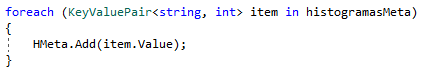
\includegraphics[width = 260pt]{Manhattan1.png}
		\caption{ }
	\end{figure} 
	
	Para obtener los elementos del diccionario que contiene los individuos de la población, se efectua otro condicional $ foreach $, por tanto sea $ i $ la cantidad de iteraciones que conlleva el recorrido de cada elemento del diccionario. Dentro de este condicional, se realizan las siguientes operaciones consideradas como valores constantes. Primeramente, mediante un contador realiza la obtención del valor del histogrma del poema meta, para luego restarle el valor que contiene el diccionario de los individuos de la población, esto gracias a las iteraciones que realiza el condicional $ foreach $. Seguidamente, en cada iteracion se van almacenando dichas operaciones en valor absoluto, además del aumento de contador que hace posible obtener los elementos de histograma meta.
	
	\begin{figure}[h]
		\centering
		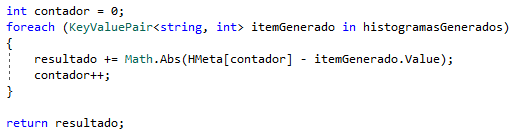
\includegraphics[width = 260pt]{Manhattan2.png}
		\caption{ }
	\end{figure}
	
	Llegado a este punto se obtiene que la complejidad del algoritmo Manhattan esta dado por $ O(p + i) $. \\
	
	
\end{itemize}

\begin{itemize}
	
	\item{\bf Distancia Chebyshev:}

	Como se pudo observar con anterioridad, la idea de la distancia Chebyshev es realizar un almacenamiento en un arreglo del valor absoluto de la resta de cada valor, por ejemplo de dos listas.
	En nuestro caso se utilizaron dos diccionarios, de los cuales, uno contendrá el histograma del poema meta, y el segundo el histograma de los individuos de la población.
	Como es evidente, para realizar esta sumatoria, es necesario recorrer e ir obteniendo cada valor de los diccionarios, por tanto, sea $ n $ la condición que conlleva la cantidad de valores contenidos
	en el diccionario del histograma del poema meta, dentro de dicho condicional se realiza una adicción a una lista que contiene valores de tipo entero de dicho histograma, por tanto, se considera operación elemental.
	
	\begin{figure}[h]
		\centering
		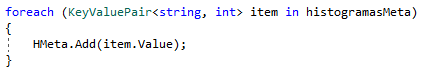
\includegraphics[width = 260pt]{Manhattan1.png}
		\caption{ }
	\end{figure}
	
	Para recorrer y efectuar la operación según la fórmula que implica la distancia Chebyshev, se realiza un condicional $ foreach $ que recorre cada valor del histograma de cada individuo de la población,
	por tanto sea $ m $ la cantidad de iteraciones según la cantidad de valores contenidos en dicho diccionario. Dentro de dicho condicional, se efectua la operación Chebyshev, donde mediante un contador
	se obtiene cada elemento de la lista anteriormente creada, que contiene el valor del histograma del poema meta; gracias a dicho condicional $ foreach $ se obtienen los valores del histograma contenidos en el
	diccionario de los individuoo de la población, entonces, se realiza la resta en valor absoluto de ambos valores, para posteriormente ser almacenados en una lista. Dichas operaciones anteriormente nombradas
	corresponden a valores constantes, por tanto, la adicción a dicha lista de la resta en valor absoluto corresponden a operaciones elementales, además del aumento del contador.
	
	\begin{figure}[h]
		\centering
		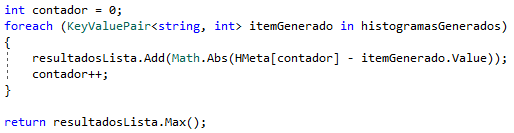
\includegraphics[width = 260pt]{Chebyshev2.png}
		\caption{ }
	\end{figure}
	
	Posteriormente, se retorna el valor máximo de la lista resultante, del cual corresponderá al mismo largo del diccionario de los individuoo de la población.
	Por tanto, se tiene que la complejidad del recorrido Chebyshev corresponde a $ O(n + 2 \cdot m) $. \\
	
\end{itemize}

\begin{itemize}
	
	\item{\bf Distancia personalizada:}
	
	De la misma forma que los dos recorridos anteriores, se tienen dos estructuras que corresponden a diccionarios, el histograma de los individuos de la población, y el histograma del poema meta correspondientemente. Nuevamente, es completamente necesario iterar sobre ambos diccionarios, ya que, lo que se pretende con este tipo de recorrido, es lograr un tipo de cruce entre el recorrido Manhattan y el recorrido Chebyshev, por lo anterior dicho, sea $ t $ la cantidad de iteraciones sobre los elementos del diccionario del histograma del poema meta, realizando en cada $ t $ iteración una inserción a una lista que contendrá el valor del histograma de cada n-gram, siendo esto último de valor constante.
	
	\begin{figure}[h]
		\centering
		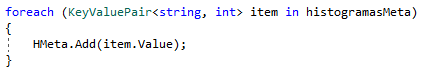
\includegraphics[width = 260pt]{Manhattan1.png}
		\caption{ }
	\end{figure}
	
	Como es de intuir, se debe recorrer el segundo diccionario para cumplir con la formula generada para este tipo de recorrido:
	{\large $ |\frac{max(x, y)}{2}| -2 $}. Por tanto, sea $ u $ la cantidad de veces en ejecutar las secuencias de código según el largo del diccionario de los individuos de la población.
	Como se puede observar, se presenta un variable acumuladora que contendrá el resultado de la distancia producidad, gracias a las $ u $ iteraciones de las operaciones. Dichas operaciones consisten en, obtener cada valor de ambos diccionarios y escoger el valor máximo de éstos que, seguidamente se realiza una división entre 2 de dicho valor máximo, y finalmente, se efectura el valor absoluto de dicho resultado con una resta de 2. Todo lo anterior dicho, se considera de valor constante, es decir, operación elemental, además del incremento del contador.
	
	\begin{figure}[h]
		\centering
		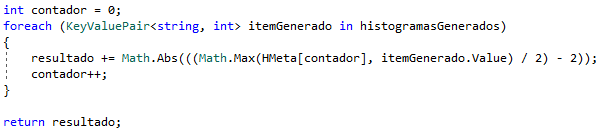
\includegraphics[width = 280pt]{DistanciaPropia2.png}
		\caption{ }
	\end{figure}
	
	Se tiene entonces que, la complejidad del algoritmo de la distancia personalizada corresponde a $ O(t + u) $. \\
	

\end{itemize}

\newpage
\section{Experimentos}
 

\begin{itemize}
	\item{\bf Comparación de duración en milisegundos entre las distancias:}  \\
	En el primer experimento se procede a evaluar la duración y rendimiento del algoritmo con respecto cada distancia implementada en el algoritmo. Cabe destacar que la cantidad de inviduos es aleatoria, por lo tanto la cantidad de veces que entra a una distancia es diferente. Sin embargo se hará un rango de milisegundos para cada distancia. 
	En primer lugar, la distancia Chebyshev de acuerdo a su procesamiento, tiene una duración de entre 2 y 4 milisegundos. Para la distancia Manhattan la duración corresponde a entre 2 y 3 milisegundos. Por último la distancia propia tiene una duración de entre 2 y 6 milisegundos. Como podemos apreciar, la distancia Manhattan tiene una menor cantidad de milisegundos empleados en el procesamiento de la distancia con respecto a las otras distancias. Esto podría deberse a que para el cálculo de la distancia Manhattan únicamente se realiza operación de resta entre los histogramas, se calcula su valor Absoluto y se suma al acumulador. Por otra parte la distancia Chebyshev requiere realizar la misma resta y calcular el valor absoluto, luego agregarlo a una lista y por último recorrer esta lista para calcular su valor máximo. Para la distancia propia, requiere calcular el valor máximo entre ambos histogramas, dividirlo por 2 y restar 2 , por último sacar su valor absoluto y sumarlo al acumulador. Por lo anterior podemos concluir que el tiempo de ejecución esta relacionado por la cantidad de operaciones que debe realizar cada distancia, siendo la Manhattan la que utiliza menos operaciones, seguida por la Chebyshev y la distancia propia que es la de mayor procesamiento. Sin embargo, a pesar de que la distancia propia tiene un promedio mayor que las otras dos distancias, esta llega a asemejarse en su valor mínimo y la pequeña diferencia entre estás no presenta mayor impacto.
	En la imagen 7 podemos apreciar gráficamente el promedio de la duración de cada distancia y su comparativa.
	
	\begin{figure}[h]
		\centering
		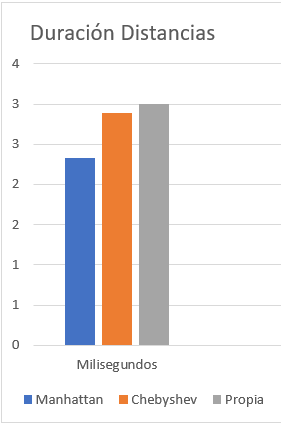
\includegraphics[width = 130pt]{comparacion.png}
		\caption{Promedio de duración de cada algoritmo }
	\end{figure}
	
	\newpage
	\item{\bf Comparación de duración en segundos del procesamiento de las diferentes cantidades de generaciones:}  \\
	En el siguiente experimento se realizará una comparación entre el procesamiento de las generaciones ingresadas por el usuario. Se evaluarán 10, 20, 30, 40 y 50 generaciones para cada una de las distancias. 
	Primeramente se realizará el procesamiento con diferentes cantidades de generaciones y la distancia Manhattan. Para el cálculo de 10 generaciones, se obtuvo una duración de 3,6 segundos, para 20 generaciones se obtuvo 4,5 segundos, las 30 generaciones dieron como resultado 9,1 segundos,  para las 40 generaciones se tienen 21.3 segundos y por último para las 50 generaciones tiene una duración de procesamiento de 34.1 segundos. De manera resumida se puede apreciar en el siguiente gráfico:
	
	\begin{figure}[h]
		\centering
		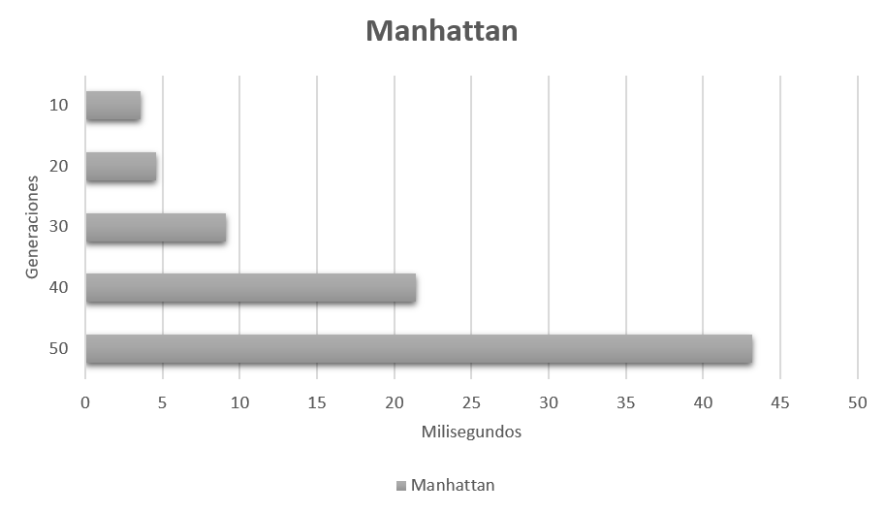
\includegraphics[width = 280pt]{manhattan.png}
		\caption{Comparanción en segundos según la cantidad de generaciones con la distancia Manhattan }
	\end{figure}
	
	
	Con la distancia Chebyshev dio los siguientes resultados: Para el procesamiento de 10 generaciones dio como resultado 5,5 segundos. Para 20 generaciones, 5,6 segundos. Siguiendo con 30 generaciones, esta dio como resultado 12,1 segundos. Para 40 generaciones tiene una duración de 18,3 segundos. Por último 50 generaciones tienen una duración de 42,9 segundos.
	
	\begin{figure}[h]
		\centering
		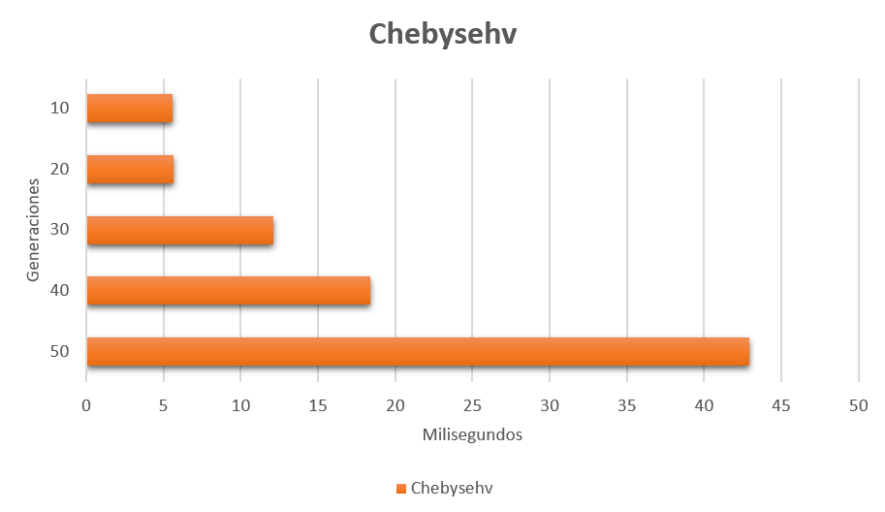
\includegraphics[width = 280pt]{chebyshev.png}
		\caption{Comparanción en segundos según la cantidad de generaciones con la distancia Chebyshev }
	\end{figure}
	
	Por último la duración de cada generación utilizando la distancia propia. 10 generaciones tienen una duración de 8,1 segundos, 20 generaciones duran 13,7 segundos, 30 generaciones tiene un tiempo de 19,8 segundos, para 40 generaciones la duración corresponde a 22 segundos y por último 50 generaciones tienen una duración de 30,9 segundos.
	
	\begin{figure}[h]
		\centering
		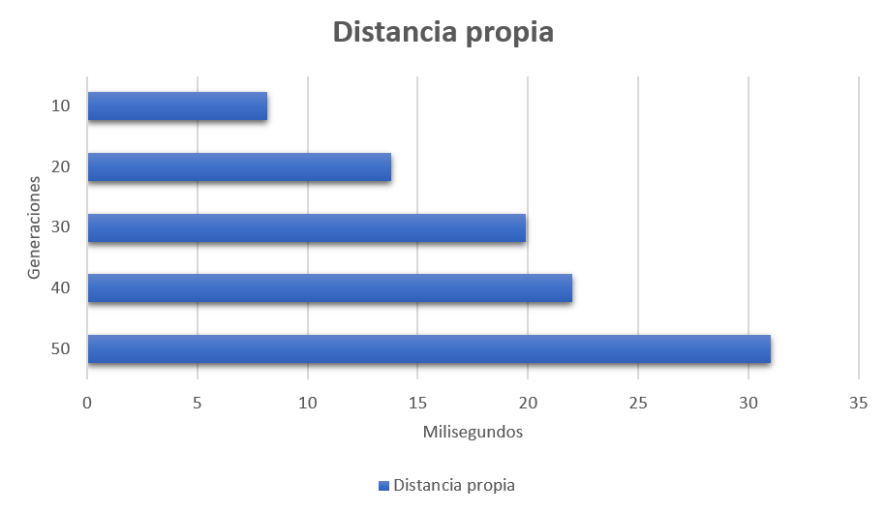
\includegraphics[width = 280pt]{propia.png}
		\caption{Comparanción en segundos según la cantidad de generaciones con la distancia propia }
	\end{figure}
	
	
	Como pudimos apreciar en las tres imágenes anteriores, el procesamiento del algoritmo genético y sus distancias tienen un crecimiento gradual, que va aumentando según aumenta la cantidad de generaciones. En la siguiente figura podemos apreciar una comparación entre estas distancias. 
	
	\begin{figure}[h]
		\centering
		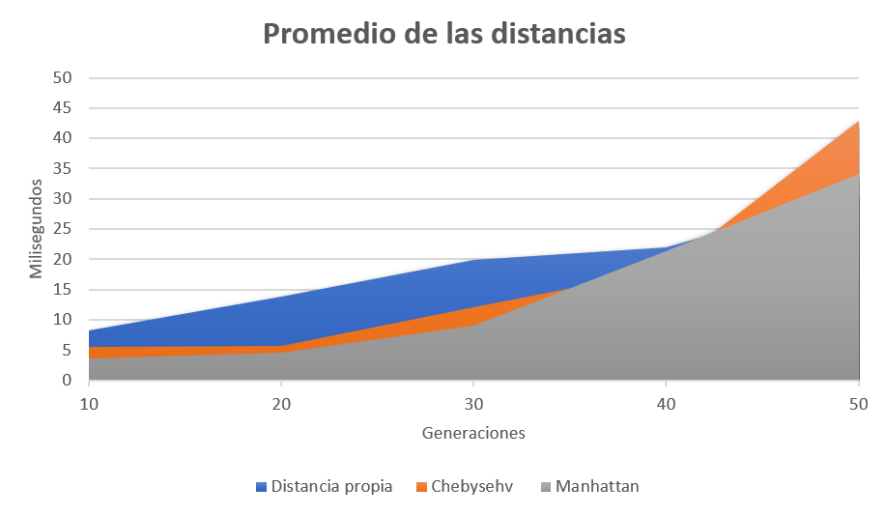
\includegraphics[width = 280pt]{resumen.png}
		\caption{Comparación en segundos entre las distancias según la cantidad de generaciones} 
	\end{figure}
	

	\newpage
	\item{\bf Comparación de la similitud de individuos generados dadas $ n $ generaciones.}\\
	
	Se pretende comparar y analizar cada proceso genético dado un número $ n $ de generaciones, donde se podrá observar la similitud entre los individuos mas prometedores según su distancia,
	con respecto al poema meta ingresado previamente.
	Primeramente, se definió la distancia Manhattan como punto de adaptabilidad para el proceso genético. En cuanto a los valores de las generaciones, se establecieron: 
	15, 50 y 100 como las cantidades de generaciones a procesar en el algoritmo genético.
	El poema meta ingresado corresponde al siguiente: 
	
	\begin{center}
		\textit{I thought that 
			I was free but it is not true \\
			A wall stands in my way to freedom \\
			Bricks, stones Masonry patterns, \\
			maybe so are the trees and rivers \\
			Colums and dams: walls of obstacles \\
			Barries, impediments, burlesque fortresses.} \\
	\end{center}
	
	
	Por tanto, el resultado obtenido con 15 generaciones corresponden a los siguientes tres individuos de la población:\\
	
	\textbf{Individuo 1:} \\
	\textit{Censured thou logicians be speak to persist greek, by my haunts damasked, time hopes? brown earth, wroth, when.}     
	
	\textbf{Individuo 2:} \\
	\textit{The bewailing, her be on or elsewhere broad bright, shall skaters slim among cronos old denies.}
	
	\textbf{Individuo 3:} \\
	\textit{Any protector breast, bricks, of take and de evening's not eagle ever fire, beauty can pipes roses no heavenly them taught last i.} \\
	

	El resultado con 50 generaciones correspondió a los siguientes individuos: \\
	
	\textbf{Individuo 1:} \\
	\textit{Lead kick spurting both shorten rivers they of sound, repose and they fortresses.}
	
	\textbf{Individuo 2:} \\
	\textit{Your wall this excellence, to all: of achilles' for sooth, something waved be free, 'ill shall small.}
	
	\textbf{Individuo 3:} \\
	\textit{One thee would amazde, pace and trees water a knee allay, though yea, born falling many shadow although falling a over.} \\
	
	El resultado con 100 generaciones correspondió a los siguientes individuos: \\
	
	\textbf{Individuo 1:} \\
	\textit{For eye and a wall though walls of bricks, but love, was free maybe free which and maybe like owls beneath friends, in dams: and rivers helpe rivers with sprawls.}
	
	\newpage
	\textbf{Individuo 2:} \\
	\textit{Kitchen pavement, or english the riddles i moan, blood floor splayed obstacles though maybe any is.}
	
	\textbf{Individuo 3:} \\
	\textit{Of it plays on when i thou be? beach: withouten shew, wrong a clearness love's with gentle the of freedom. their now birds one one kind quick know to free absent rankes wall stands.} \\
	
	Claramente, se puede apreciar que con forme sea mayor el número de generaciones, se incrementa el número de posibilidades en cuanto a la similitud de las palabras de los poemas generados, 
	sin embargo, como es de intuir, existirá algún número de generaciones elevado donde los genes de los individuos se pierdan, por tanto dicha similitud iría decreciendo con respecto
	a la población, apezar de que su distancia se mantenga o disminuya, dependiendo de que tan factible son dichos individuos por medio de las probabilidades que se implementaron. 
	Por tanto, consideramos que un buen número de $ n $ generaciones ronda un promedio de 100. Y por su puesto, las sintaxis de los poemas generados, en la mayoria de las ocaciones, 
	carecen de sentido alguno.
\end{itemize}

\newpage
\section{Conclusión}
	En este proyecto se aprendió a elaborar, en el lenguaje de programación C\# un programa generador de texto a partir de un poema meta dado. Se estudió el campo de los algoritmos genéticos los cuales permiten el desarrollo de individuos y obtener una población más óptima con cada generación. Además se aprendió el concepto de distancia, la cual permite el cálculo de similitudes entre individuos de una población y las diferentes operaciones con las cuales se maneja cada distancia. Debido a lo anterior se logró desarrollar una distancia con una operación propia, la cual debido a los experimentos a los que fue sometida presenta una similitud frente a las otras dos distancias. Para dichos experimentos que se realizaron se encuentran, la comparación en milisegundos de la duración de las tres diferentes distancias y se encontró que la distancia Manhattan es la de mayor velocidad por encima de la distancia Chebyshev y la propia, sin embargo esta diferencia fue mínima. Además se hizo la comparación de que tan grande es la diferencia en segundos entre el procesamiento de diferentes cantidades de generaciones para cada una de las distancia. En adición a la sección de experimentos se comparó y analizó cada proceso genético dado un número de generaciones, donde se podrá observar la similitud entre los individuos mas prometedores según su distancia, con respecto al poema meta ingresado previamente.
	



\end{document}


